\documentclass[border=4pt]{standalone}
\usepackage{tikz}
\usetikzlibrary{calc}

\begin{document}
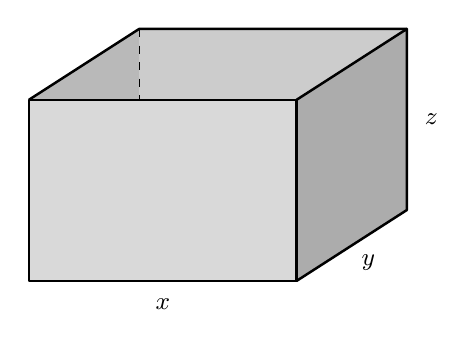
\begin{tikzpicture}[x=1cm, y=1cm, font=\small, line join=round]
    % caja abierta: frente 3.4 x 2.3, profundidad (1.4, 0.9)
    \coordinate (A) at (0,0); \coordinate (B) at (3.4,0);
    \coordinate (C) at (3.4,2.3); \coordinate (D) at (0,2.3);
    \coordinate (d) at (1.4,0.9);
    % caras interiores
    \fill[gray!55] (D) -- ($(D)+(d)$) -- ($(A)+(d)$) -- (A) -- cycle;
    \fill[gray!40] ($(A)+(d)$) -- ($(B)+(d)$) -- ($(C)+(d)$) -- ($(D)+(d)$) -- cycle;
    % cara lateral derecha y frontal
    \fill[gray!65] (B) -- ($(B)+(d)$) -- ($(C)+(d)$) -- (C) -- cycle;
    \fill[gray!30] (A) -- (B) -- (C) -- (D) -- cycle;
    \draw[line width=0.9pt] (A) -- (B) -- (C) -- (D) -- cycle;
    \draw[line width=0.9pt] (B) -- ($(B)+(d)$) -- ($(C)+(d)$) -- (C);
    \draw[line width=0.9pt] (D) -- ($(D)+(d)$) -- ($(C)+(d)$);
    \draw[dashed] ($(D)+(d)$) -- ($(D)+(d)+(0,-0.9)$);
    \node[below=3pt] at (1.7,0) {$x$};
    \node[below right] at ($(B)+0.5*(d)$) {$y$};
    \node[right=3pt] at ($(B)+(d)+(0,1.15)$) {$z$};
\end{tikzpicture}
\end{document}
